\chapter{Proposed Solution: Workflow-First Deployment via Function Registry Resolution}
\label{ch:proposed_solution}

In OmniFlow, a \texttt{call} step is an HTTP request with a concrete \texttt{method}, \texttt{host}
and \texttt{path}. The proposed solution lets the developer name a function they own instead,
through \texttt{internalFunction(name, deploymentDescriptorPath)}, and resolves its endpoint at
deployment time. A single, workflow-first deployment then resolves (or, if needed, deploys) the
functions and deploys the workflow.

Section~\ref{sec:components-architecture} presents the components the integration adds, and
Section~\ref{sec:dsl-extensions} the \texttt{internalFunction} construct and the concepts it relies
on. Section~\ref{sec:resolution-cascade} presents the three-level resolution ladder,
Section~\ref{sec:design-rationale} why OmniFlow drives QuickFaaS, and
Section~\ref{sec:developer-workflow} the procedure from the developer's point of view.

\section{Components Architecture}
\label{sec:components-architecture}

Figures~\ref{fig:architecture-before} and~\ref{fig:architecture-after} contrast the two tools
before and after the integration. Before it, the developer deploys each function with QuickFaaS,
reads its endpoint and copies it into the workflow definition
(Section~\ref{sec:int_cha_int_uni_multi}); QuickFaaS has no AWS support.

\begin{figure}[tbp]
  \centering
  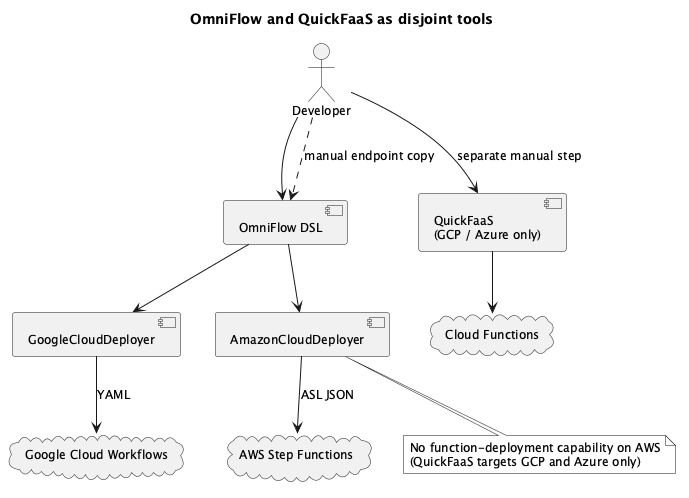
\includegraphics[width=0.85\textwidth]{images/architecture/architecture-before.png}
  \caption{OmniFlow and QuickFaaS operate as two disjoint tools.}
  \label{fig:architecture-before}
\end{figure}

After it, one workflow definition drives both deployments. Each provider deployer delegates call
resolution to a provider-specific resolver, backed by a registry file of its own that maps logical
names to invocation metadata. QuickFaaS gains an \texttt{AwsProvider}, so a function can be
deployed on demand to AWS Lambda through the same subprocess mechanism used for GCP.

\begin{figure}[tbp]
  \centering
  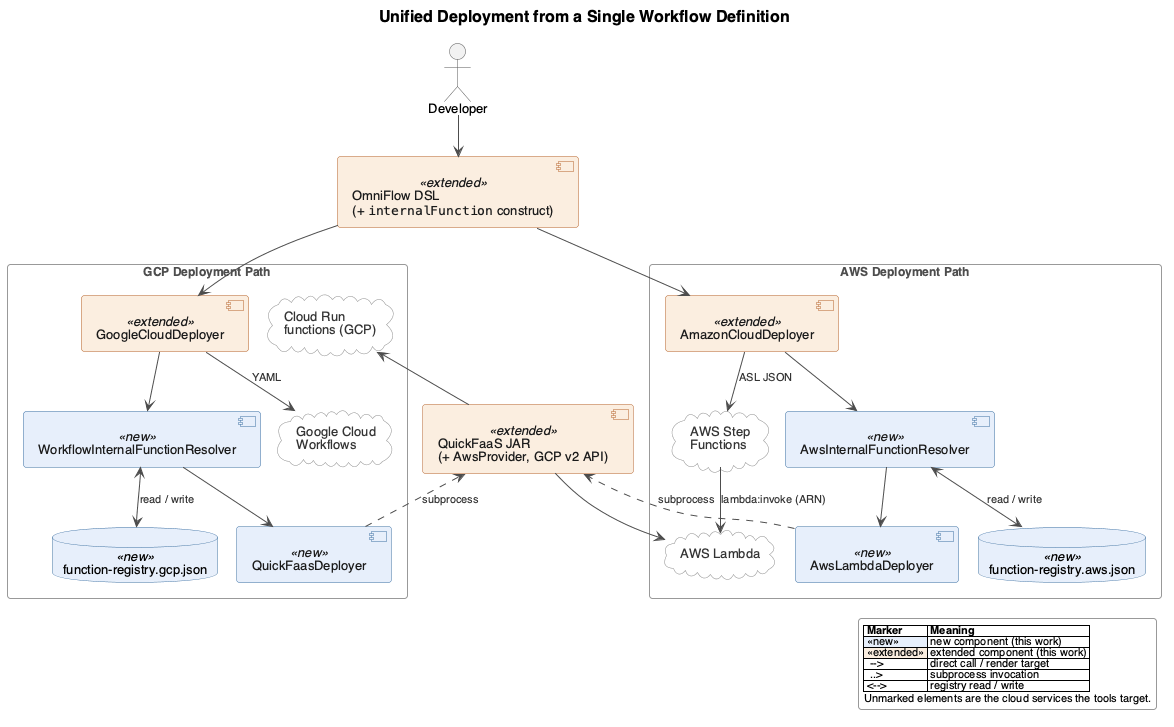
\includegraphics[width=\textwidth]{images/architecture/architecture-after.png}
  \caption{Unified deployment driven from a single workflow definition. Components marked as new/extended are the contribution of this work.}
  \label{fig:architecture-after}
\end{figure}

The end-to-end flow is:
\begin{enumerate}
  \item the developer defines the workflow and one QuickFaaS descriptor per internal function;
  \item OmniFlow walks the workflow tree and finds each internal call;
  \item for each internal call, it resolves the endpoint from the registry, discovers it on the
  provider, or deploys the function through QuickFaaS;
  \item metadata obtained by discovery or deployment, or refreshed after drift, is written to the
  registry;
  \item the resolved workflow is rendered and deployed.
\end{enumerate}
Calls with a literal endpoint bypass the registry.

\section{DSL Extensions}
\label{sec:dsl-extensions}

Figure~\ref{fig:call-step-model} shows the extended \texttt{call} step. A \texttt{CallContext}
carries either the literal \texttt{host} and \texttt{path} or, new in this work, an
\texttt{InternalFunction} with a logical \texttt{name} (the \texttt{functionRef}) and an optional
\texttt{deploymentDescriptorPath}. The two forms are mutually exclusive: for an internal call,
\texttt{host} and \texttt{path} are injected at deployment time. Extending the existing step, rather
than adding a step type, keeps the same HTTP vocabulary for both.

\begin{figure}[tbp]
  \centering
  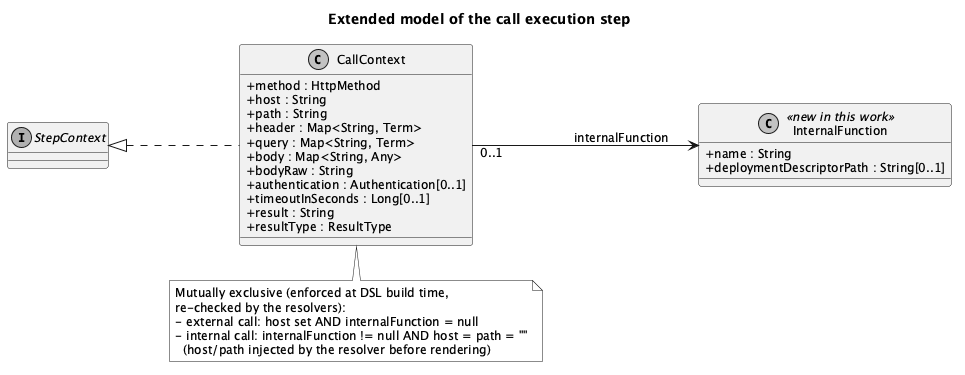
\includegraphics[width=0.8\textwidth]{images/dsl-extension/call-step-model.png}
  \caption[Extended model of the \texttt{call} execution step.]{Extended model of the
  \texttt{call} execution step, with the mutually exclusive \texttt{internalFunction} association
  added in this work.}
  \label{fig:call-step-model}
\end{figure}

\paragraph{Internal and external functions.}
A function whose code the workflow developer owns and may deploy is \emph{internal}, declared with
\texttt{internalFunction}. A function or API the developer does not own is \emph{external}: it is
called through a literal \texttt{host}/\texttt{path}, never deployed by QuickFaaS and never
recorded in the registry.

\paragraph{Function reference (\texttt{functionRef}).}
A stable logical name for an internal function (e.g., \texttt{"fraud-check"}), used in the
workflow, the registry and the deployment descriptor. It is not an endpoint: OmniFlow binds it to
one at deployment time.

\paragraph{Function Registry.}
A file per provider that maps each \texttt{functionRef} to the values needed to invoke it
(Listing~\ref{lst:registry-structure}). \texttt{updatedAt} records the last write. The key is the
bare reference, or \texttt{"region/functionRef"} when the same name exists in more than one region.
Each entry has two fields: \texttt{serviceName}, the function's name on the provider (on GCP, the
full resource name of the Cloud Run service), and \texttt{url}, what the rendered workflow invokes:
the HTTPS endpoint on GCP, split by the resolver into \texttt{host} and \texttt{path}, and the ARN
on AWS, used for a native Lambda invocation. No credentials are stored. The integration writes both
files, by default in the working directory.

\begin{lstlisting}[caption={Example registry files, one per provider (registry-managed functions only).},label={lst:registry-structure},basicstyle=\ttfamily\footnotesize,breaklines=false]
function-registry.gcp.json:
{
  "updatedAt": "2026-02-12T18:40:00Z",
  "functions": {
    "fraud-check": {
      "serviceName": "projects/proj/locations/us-east1/services/fraud-check",
      "url": "https://fraud-check-a1b2c3d4e5-ue.a.run.app"
    }
  }
}

function-registry.aws.json:
{
  "updatedAt": "2026-02-12T18:40:00Z",
  "functions": {
    "hello-lambda-fn": {
      "serviceName": "hello-lambda-fn",
      "url": "arn:aws:lambda:eu-west-1:123456789012:function:hello-lambda-fn"
    }
  }
}
\end{lstlisting}

Listing~\ref{lst:call-step-internal} shows an internal call. It has no \texttt{host} or
\texttt{path}: \texttt{internalFunction} gives the \texttt{functionRef} and the QuickFaaS
descriptor, which is read only if the ladder reaches Level~3. The step says which function to
call; the deployment determines where it is.

\begin{lstlisting}[language=Kotlin,caption={Call step declared via \texttt{internalFunction} (excerpt of the \texttt{FraudPipeline} workflow, Listing~\ref{lst:wf-fraudpipeline-full}).},label={lst:call-step-internal}]
step {
  name("fraud-check")
  description("Call the fraud-check function")
  context(call {
    method(GET)
    internalFunction("fraud-check", "./deploy/fraud-check.json")
    result("fraudResult")
  })
}
\end{lstlisting}

\paragraph{Deployment descriptor and code file.}
An internal function is deployed from the QuickFaaS descriptor of
Listing~\ref{lst:quickfaas_json_config} and the code file named in its \texttt{functionFile}. Two
fields matter beyond deployment: \texttt{function.name} must equal the \texttt{functionRef}, since
the resolver looks the deployed function up by that reference (Section~\ref{sec:walkthrough}); and
\texttt{function.location} fixes the region the registry entry points at. The AWS variant adds an
\texttt{iamRoleArn} field for the Lambda execution role (Listing~\ref{lst:aws-descriptor}).

\section{The Resolution Ladder}
\label{sec:resolution-cascade}

Each internal call is resolved independently by a three-level ladder that stops at the first level
that succeeds. The cheapest, least intrusive action comes first; a deployment is the last resort.

\begin{enumerate}
  \item \textbf{Level~1 (Registry).} The registry is looked up for the \texttt{functionRef}. A hit
  is validated with a single lookup of the live function (the Cloud Run service on GCP, the Lambda
  function on AWS) where the entry records it. A changed endpoint refreshes the entry. A deleted
  function is searched for in the other regions: if found, the entry is replaced; if not, the entry
  is removed and the deployment aborts.
  \item \textbf{Level~2 (Provider discovery).} On a registry miss, the function is looked up on
  the provider: across the project's Cloud Run regions on GCP, and across every region enabled for
  the account on AWS (\texttt{GetFunction}). A \texttt{"region/functionRef"} reference takes a
  single lookup. A function found, for instance one deployed outside the integration, is recorded
  in the registry and used, without a deployment.
  \item \textbf{Level~3 (QuickFaaS deployment).} Only when the function is absent from both the
  registry and the provider, and the call supplies a \texttt{deploymentDescriptorPath}, does
  QuickFaaS deploy it. The returned metadata is registered and used. Without a descriptor, the
  deployment aborts with a diagnostic naming the function.
\end{enumerate}

The ladder is \emph{idempotent}: re-deploying a workflow resolves from the registry or the provider
and never redeploys an existing function. It is \emph{safe by default}: validation and discovery
never change the provider, and a deployment requires an explicit descriptor and confirmed absence
(a deployment also grants invocation permissions and, on AWS, sets up an execution role;
Section~\ref{subsec:omniflow-aws-deployer}). And it is \emph{observable}: each level reports whether
a call was served from the registry, discovered or deployed. Chapter~\ref{cha:impl} describes the
implementation.

\paragraph{Static binding.}
The ladder runs only at deployment. The resolved endpoint is written into the rendered workflow
(the \texttt{url} of an HTTP call in Cloud Workflows, the \texttt{FunctionName} of a
\texttt{lambda:invoke} task in Step Functions), and the deployed workflow never consults the
registry. If an endpoint changes afterwards, the workflow keeps calling the old one until it is
deployed again, when Level~1 detects the change. Endpoints change rarely: updating a Lambda's code
keeps its ARN, and redeploying a Cloud Run function under the same name and region keeps its URL.
They change when a function is recreated under another name, region, account or project. Run-time
resolution is outside the scope of this work.

\paragraph{Provider and region scope.}
Every provider resource lives in a \emph{region} (e.g., \texttt{eu-west-1} on AWS,
\texttt{europe-west1} on GCP), which is part of its identity. Each deployment targets one provider
(Section~\ref{sec:int_cha_int_uni_multi}), but the workflow and its functions need not share a
region, and the developer need not say where a function is: Level~2 searches every region,
starting with the workflow's own, where co-location reduces latency and cost. On AWS, a Lambda must
be in the region of the S3 bucket that holds its code, so the AWS deployer takes its region from
that bucket (Section~\ref{subsec:omniflow-aws-deployer}).

\section{Design Rationale: Embedding Function Deployment in OmniFlow}
\label{sec:design-rationale}

\paragraph{Why OmniFlow orchestrates QuickFaaS.}
Only OmniFlow knows the workflow: it owns the deployment entry point and the workflow tree, and
therefore which functions to resolve. QuickFaaS works on one function at a time and has no notion
of a workflow. OmniFlow therefore drives QuickFaaS, in a one-shot, client-side action at deployment
time. To keep the tools decoupled, function deployment sits behind a strategy interface with one
implementation per provider (Section~\ref{sec:function-registry}), each invoking QuickFaaS as an
external process. QuickFaaS is reused as-is, with its own repository, Gradle build and
Kotlin~1.6.20 toolchain.

\paragraph{Why not two communicating services.}
Neither tool is a service: OmniFlow is a library invoked during a build, QuickFaaS a desktop
application with no network API. Running them as services would mean re-architecting and operating
both, the additional runtime layer this work avoids (Section~\ref{ch:related-works}), and carrying
local cloud credentials across a trust boundary, with no benefit for a deployment on one machine.

\paragraph{Trade-off of the subprocess.}
OmniFlow places the descriptor and function source next to the QuickFaaS JAR, launches it with
\texttt{java\ -jar}, and detects success from the exit code and a marker on its output. This reuses
QuickFaaS's headless entry point unchanged, but it is the most brittle part of the integration: it
couples the two builds through a JAR path and parses the child's output. Invoking QuickFaaS
in-process as a library would remove the process boundary while keeping the same model; it is
future work (Chapter~\ref{cha:conclusions}).

\section{Developer Procedure for Deploying a Workflow}
\label{sec:developer-workflow}

Consider the \texttt{FraudPipeline} workflow (Listing~\ref{lst:wf-fraudpipeline-full}), with one
internal and one external call. For the internal \texttt{fraud-check}
(Listing~\ref{lst:call-step-internal}), the developer writes a QuickFaaS descriptor and the code file
it names, and chooses a \texttt{functionRef}. Reading the registry shows which references are in
use, but is not needed for a new function. The external step (Listing~\ref{lst:wf-external-part})
calls a partner API through a literal \texttt{host}/\texttt{path}, and needs no descriptor.

\begin{lstlisting}[language=Kotlin,caption={External call of the \texttt{FraudPipeline} workflow (excerpt of Listing~\ref{lst:wf-fraudpipeline-full}).},label={lst:wf-external-part},basicstyle=\ttfamily\small,breaklines=false]
step {
  name("external-risk-api")
  description("Call the partner risk-scoring API")
  context(call {
    method(POST)
    host("api.partner.example")
    path("/v1/risk-score")
    result("riskResult")
  })
}
\end{lstlisting}

\subsection{Walkthrough of an Integrated Deployment}
\label{sec:walkthrough}

Suppose \texttt{fraud-check} has never been deployed and there is no registry. OmniFlow first
bootstraps the registry (on GCP by listing the project's HTTP-invocable services, on AWS by listing
the Lambda functions in every enabled region), then walks the workflow tree. The resolver skips
\texttt{external-risk-api}. For \texttt{fraud-check}, Level~1 misses, Level~2 misses, and Level~3
runs because a descriptor was supplied: QuickFaaS deploys the function, its endpoint (a URL on GCP,
an ARN on AWS) is written to the registry under \texttt{fraud-check}, and injected into the step.
OmniFlow then renders and deploys the workflow.

On a second deployment, \texttt{fraud-check} is a Level~1 hit: no descriptor is read and nothing is
redeployed. Had the function been recreated at a new endpoint, Level~1 would bind the call to it,
with no change to the workflow definition.

\paragraph{Error and edge cases.}
All fail fast, before any artifact is rendered:
\begin{itemize}
  \item \textbf{Unresolvable function:} absent from the registry and the provider, with no
  descriptor. The deployment aborts, naming the function.
  \item \textbf{Ambiguous reference:} a bare \texttt{functionRef} that matches more than one region.
  The deployment aborts and asks for the \texttt{"region/functionRef"} form.
  \item \textbf{Both forms on one call:} \texttt{internalFunction} together with
  \texttt{host}/\texttt{path} is rejected when the DSL is built and again at resolution.
  \item \textbf{Stale binding:} a registry entry whose function no longer exists and cannot be
  rediscovered. The entry is removed and the deployment aborts, even if a descriptor is supplied,
  rather than bind the workflow to a dead endpoint.
\end{itemize}

One misconfiguration is not caught beforehand: a \texttt{functionRef} different from the
descriptor's \texttt{function.name}. QuickFaaS deploys the function under the descriptor's name,
while OmniFlow waits for one named after the \texttt{functionRef}; the wait times out and the
deployed function is not registered.
